% !TEX root = main.tex
\chapter{Airfoils and Inverted Wings}

Achieving a large negative lift coefficient $C_L$ can be done in many ways. Inspecting race cars throughout the years show that airfoils have been used as early as 1966 when Jim Hall attached a rear wing to his Chaparral 2E \cite{hucho}. Since then, the inverted wings have been a staple in the racing industry with various three dimensional geometries affecting the overall performance even further.

This chapter covers the pressure distribution of various airfoils, the selection criterions of the competition, three dimensional geometrical effects and the tools of the optimization trade.

\section{Airfoil theory}

  An airfoils is the 2-dimensional cross section of a wing, that's characteristic of the wing's lifting characteristics. It is important to know the nomenclature: The leading edge is  the most forward point of the wing, the trailing edge is the most rearward point of the wing. Camber is how much the wing ''flexes''.




  \fxnote{Mostly laminar flow, boundary layer mustn't trip or create bubbles,}
Theory of airfoils from katz book, to be written tuesday 19.



  \subsection{Pressure distribution}

  \subsection{Lift and Drag Coefficient}

  Lift coefficient:
  \begin{align}
    C_L &= C_{L_\alpha} (\alpha + \alpha_{L_0})
    \intertext{where $\alpha$ is the lift per angle of attack in radians, $alpha_{L_0}$ is the airfoil's camber, which acts as a additional angle of attack effect, also in radians. $C_{L_\alpha}$ is given by:}
    C_{L_\alpha} &= \frac{2}{1+\frac{2}{\AR}} \label{eq:liftperAR}
  \end{align}

  \fxnote{something about Navier Stokes equations.}

  \subsection{Which parameters does an airfoil have? What can we change}

  \subsection{Angle of Attack}

  \subsection{Ground Effects}\fxnote{unsure}

  \subsection{Aspect Ratio and End Plates}

    An important identifyer when describing an actual finite wing is, apart from chord length and airfoil design, the width. The definition used for describing the physical span is called Aspect Ratio, and for a rectangular wing is:
    \begin{align}
        \AR_\text{actual} &= \frac{b}{c}
        \label{eq:ARactual}
    \end{align}
    Where $b$ is the width of the wing and $c$ is the chord length.

    \begin{figure}
      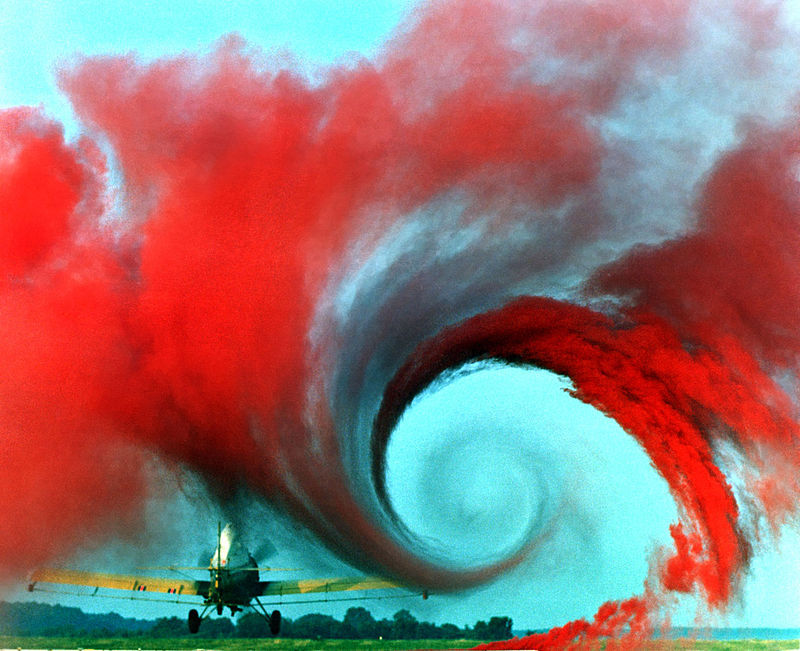
\includegraphics[width=\textwidth]{trailingtipvortex}
      \caption{The trailing tip vortex is clearly seen to the right. The . Thanks to the NASA's Wake Vortex Study for the photo \cite{nasatipvortex}.}
      \label{fig:trailingtipvortices}
    \end{figure}

    The effect of having a finite length is very important in race aerodynamics. As pressure is lowered and increased on the different sides, air is going to travel around the edge of the wing in a rolling motion. This creates a vortex, which is shown in figure \ref{fig:trailingtipvortices}. The phenomenon is called tip vortices, and the magnitude of the vortex is proportional to the lift coefficient of the wing. The area these vortices cover is very large and for wings with a small span will greatly reduces the lifting powers.

    These vortices are created by an effect called \emph{downwash} when talking aeroplanes. As the wing bends the air slightly downwards, it creates an opposite force due to Newton's second law which is lift. However, the sheet of air that passes over the length of the wing has a downward velocity component and will thus force air in that direction. This presses other air out of the way, allowing air above it to rush downwards to fill the gap. The same phenomenom is what happens at the edge of the wing, and again is what is shown in figure \ref{fig:trailingtipvortices}. When the wing \emph{bends} the airflow downward, drag is induced. While drag is almost negligible in our case, it is never wanted \cite{peterkampf}. For an elliptical wing, the induced drag coefficient is given by:

    \begin{align}
      C_{d_\text{induced}} &= \frac{C_L^2}{\epsilon \pi \AR }
    \end{align}
    Where $\epsilon = 1$ for an ellipse, and generally $\epsilon < 1$ for anything else. For a rectangular wing, $\epsilon = 0.7$ \cite{nasainduceddrag}.

    A way to combat this phenomenon is the addition of end plates. End plates adds a virtual additional length by adding a physical wall between the low- and high pressure surfaces. The vortices that usually go around the wing and reduce lift is severely hindered. A corrected aspect ratio can be found for wings with side plates as:
    \begin{align}
      \AR &= \AR_\text{actual}\left(1+1.9\frac{h}{b}\right) \label{eq:endplates}
    \end{align}
    where $h$ is the height of the end plate, and $b$ is the width of the wing as in equation \ref{eq:ARactual} \cite{jkatz}. The addition of end plates gives an increased aspect ratio. Inserting this back into \ref{eq:liftperAR} shows that end plates yields an increase in lift.
